\section{Coordinate Descent for MeerKAT Data}
The most basic cd algorithm for image reconstruction

Tries to minimize the L1 norm of the image

\begin{equation}
	\underset{X}{minimize} \: \left \| V - F^{-1}X \right \|_2^2 + \lambda \left \| X \right \|_1 \\
\end{equation}

\begin{lstlisting} 
def coordinate_descent(V_residual, X, lambda):
	for i in pixels_row:
		for j in pixels_column:
			x_old = X[i, j]
			fourier_column = calculate_fourier_transform(i, j)
			fr = real(fourier_column)
			fi = imag(fourier_column)
			rr = real(V_residual)
			ri = imag(V_residual)
			
			#find apex
			a = sum(fr**2 + 2*fr*fi + fi**2)
			b = sum(fr*rr + fr*ri + fi*rr + fi*ri)
			x_new = b / a + x_old
			
			x_new = shrink(x_new, lambda)
			X[i, j] = x_new
			V_residual = V_residual - fourier_column * (x_new - x_old)
\end{lstlisting}\label{cd:basic}

How the algorithm works, shrinkage. 

Good points: Uses exact fourier transform. Assuming all other coordinates are fixed, we find the optimum. If the coordinates are independent, we converge faster. Heuristics can be used.

If we do not reconstruct the image $X$ directly, but in a different space. In this work, starlets were used. The next section \ref{cd:starlets} describes starlets in more detail.

Calculates the full Fourier Transformation matrix. Only changes a subset of the image. Active set heuristic after a full run. This is still impractical for meerKAT data size. Since we use starlets, there is a heuristic where we never need to calculate the full Matrix $F^{-1}$. This heuristic is described in section \ref{cd:heuristic}



\subsection{Starlets Regularization} \label{cd:starlets}
Starlet is a multi-scale wavelet representation which were specifically developed for astronomy.

Over-complete representation. More starlets than there are pixels. Sparse representation, the number of non-zero starlets is smaller than the number of pixels

Starlets as a series of convolutions.

Forward transform, from image to starlets

From Starlets to image

\subsection{Active set heuristic with Starlets}\label{cd:heuristic}
Even though the starlets are an over-complete dictionary, they have an approximate transform from image to starlet space. For Coordinate Descent, this can be used as a active set heuristic: We try to find the coefficients which are likely to be non-zero. This helps us so we do not need to calculate the whole matrix product $F^{-1}D$. We only use columns that are likely to be not zero.

(Image of the starlet level zero)
The higher the number, the more likely this component is to be non-zero. It is essentially a probability distribution for which starlet components are non-zero.

Stupid approach with line search. Could be done more efficiently by using the histogram of the starlet level.

\subsection{Implementation}
coordinate descent with active set heuristic


\subsection{Results on Simulated Data}

\subsubsection{Point Sources}

\subsubsection{Gaussian and Point Sources}

\begin{figure}[h]
	\centering
	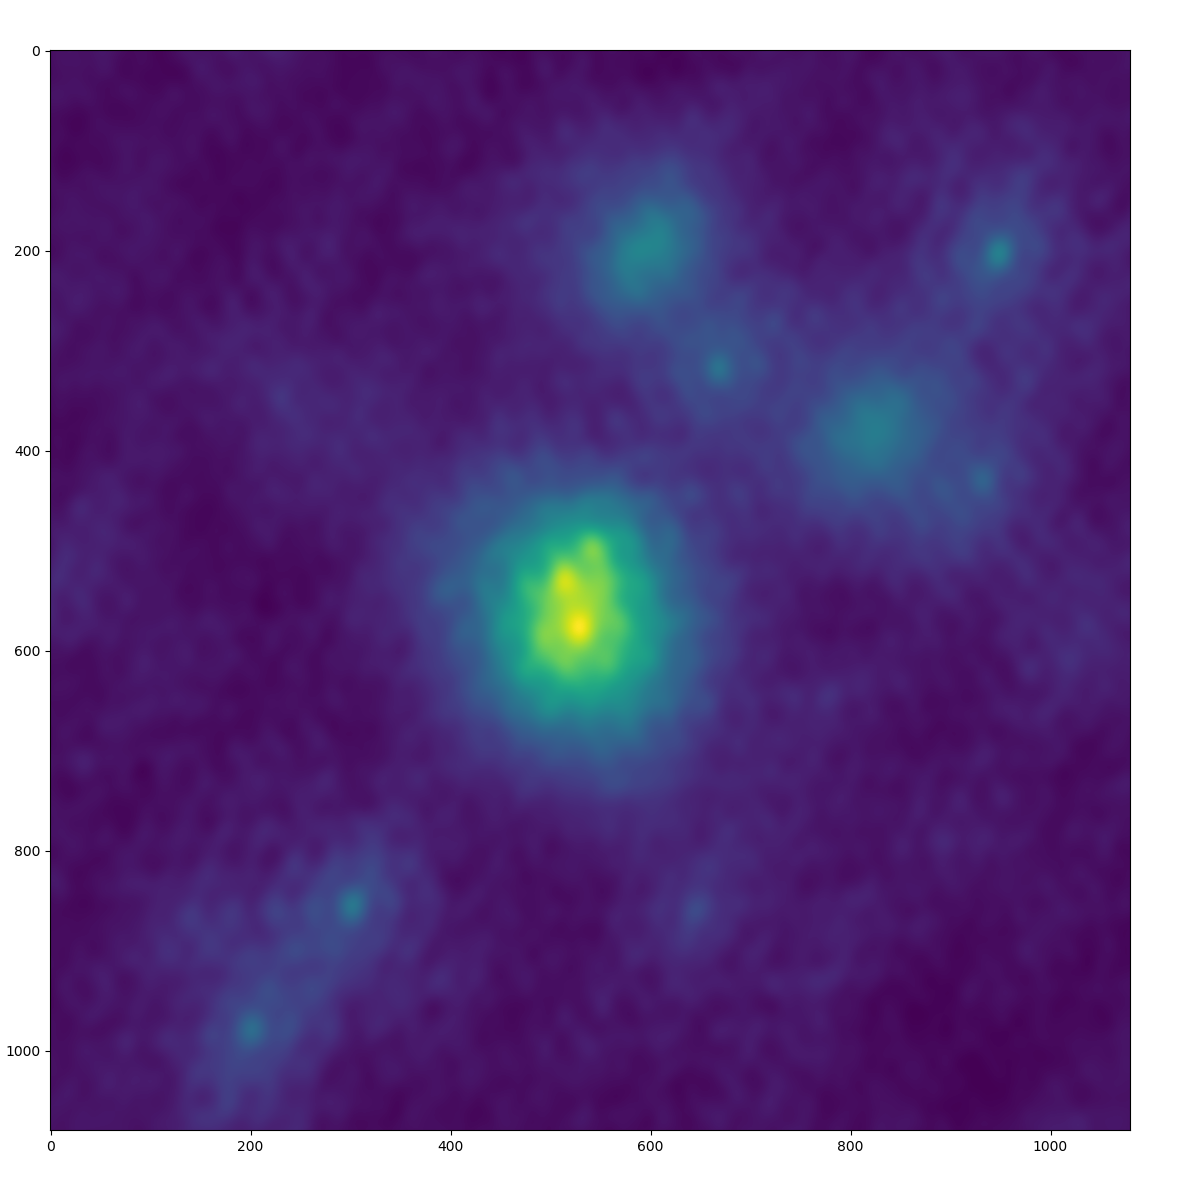
\includegraphics[width=0.5\linewidth]{./chapters/05.algorithms/results/sim00_mixed_sources_dirty.png}
	\caption{Dirty Image}
	\label{alg:gauss:dirty}
\end{figure}

\begin{figure}[h]
	\centering
	\begin{subfigure}[b]{0.45\linewidth}
		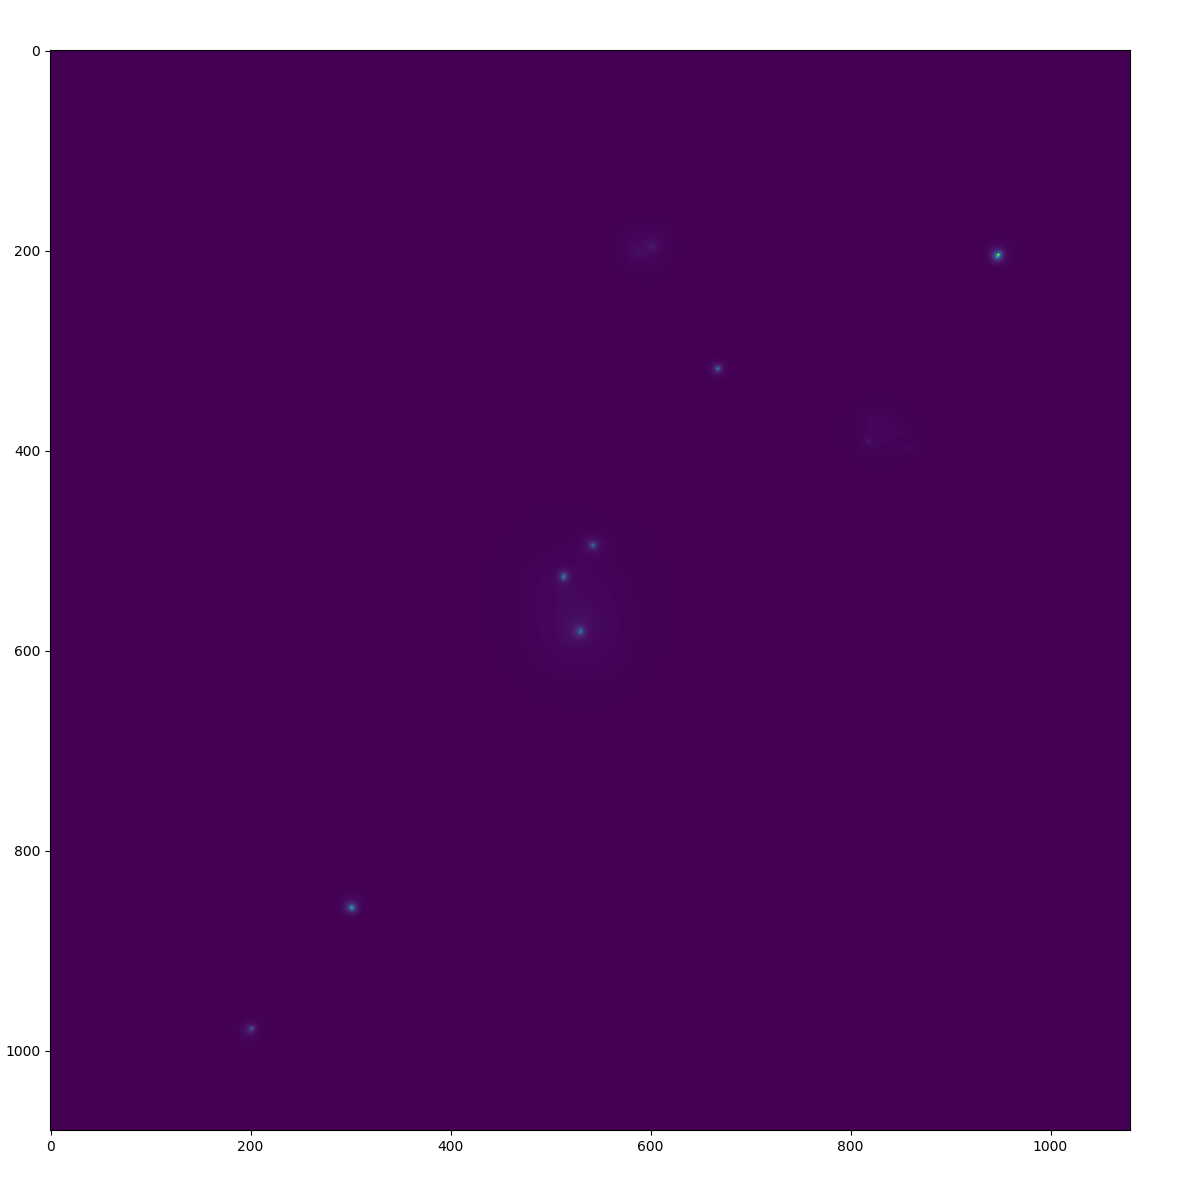
\includegraphics[width=\linewidth]{./chapters/05.algorithms/results/image.png}
		\caption{Reconstruction after one full iteration}
		\label{results:g55:nrao:rec}
	\end{subfigure}
	\begin{subfigure}[b]{0.45\linewidth}
		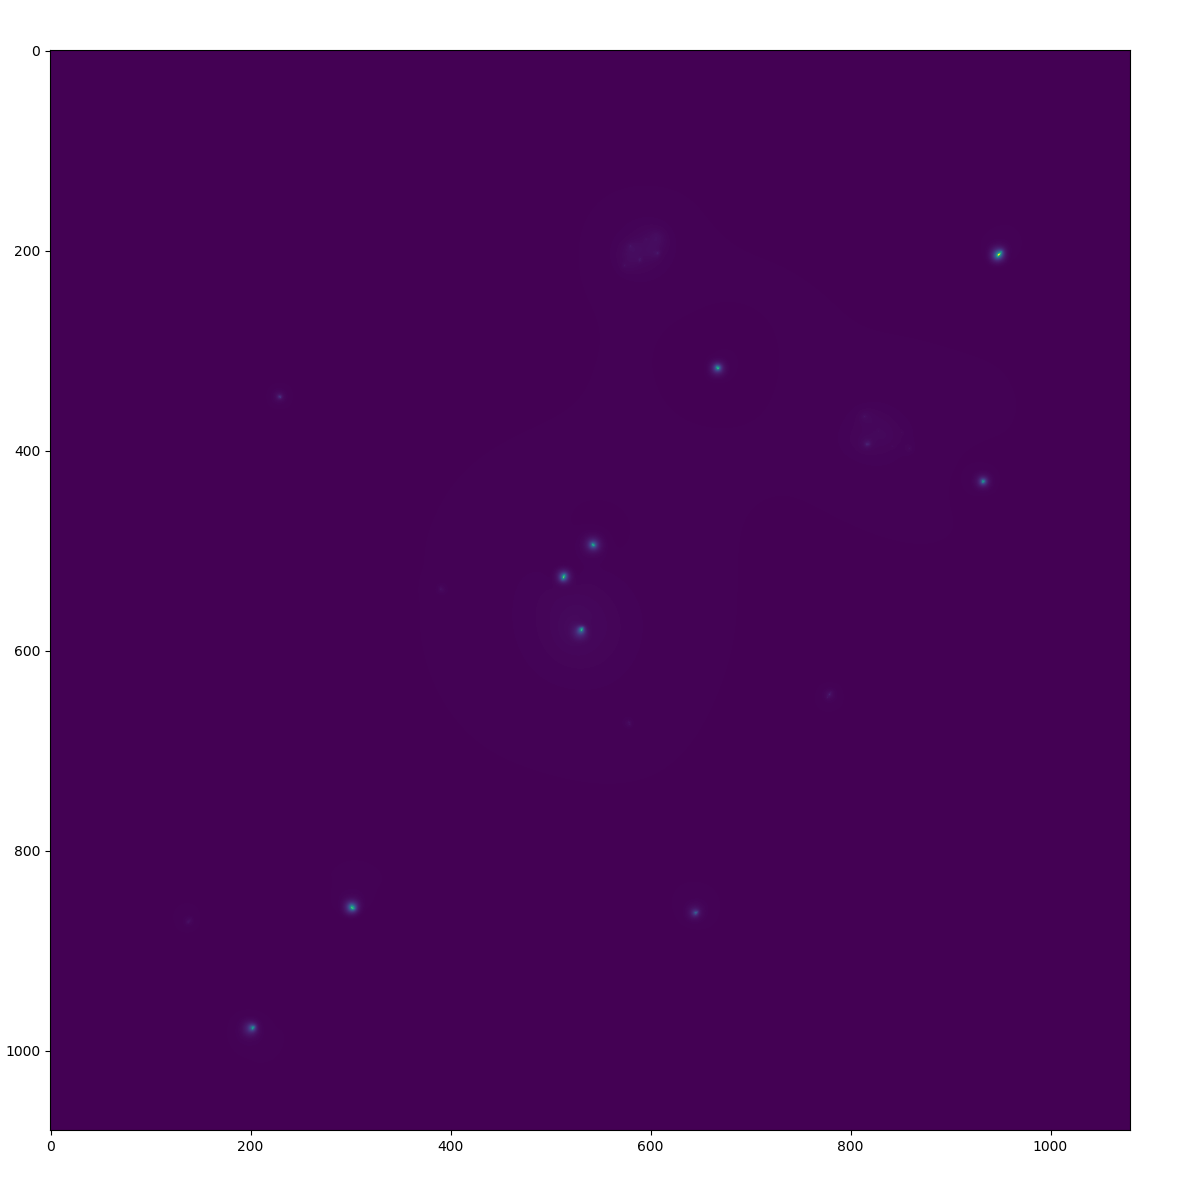
\includegraphics[width=\linewidth]{./chapters/05.algorithms/results/image4.png}
		\caption{Reconstruction after 4 Full iterations}
		\label{results:g55:nrao:dirty}
	\end{subfigure}
	\caption{}
	\label{results:g55:nrao}
\end{figure}

\subsection{Scalability estimates with ideal heuristics}
Bunch of heuristics. There are a lot of little ways to optimize this algorithm. The question is, is it worth going further and try to improve the algorithm further. So we want to estimate the lower bound of the algorithm.

Convergence is hard to determine in general. Following simplified assumptions were made: We have a heuristic with oracle performance. It returns only the locations of $\alpha$ in constant time. Furthermore, we assume all axes are independent from each other, only one descent per non-zero axis is necessary.

$S$


$res * starlet = M$
descent:
$gen fcol = 3*M$
$a = 3 * M$
$b = 4 * M$
$residuals, fcol*diff =  M$

$total_mit_gencol = 11M$

total CD = $S * 11M + 2M * starlets$

$S$ depends on the image content directly. For example if the image contains 15 point sources and five Gaussian extended emissions, then $S$ equals 20 non-zero components (if we assume the Gaussian sources require only one starlet for representation). Coordinate Descent therefore is independent of the image size $N$. It solely depends on the size of the measurements $M$, and the number of non-zero components in the dictionary $S$. 

It does not use any approximation for the fourier transform.



(Cite New W-stacking approach)
Nufft: $M + 2N log 2N$
W-stacking = $M + W*(2N log 2N + 2N) + N log N$
Deconvolution = ??

The major cycle algorithm depends on more parameters. Assumptions were made in favor of Coordinate Descent.

the number of w-stacks $W$. If this is the case

